\begin{minipage}{0.115\textwidth}
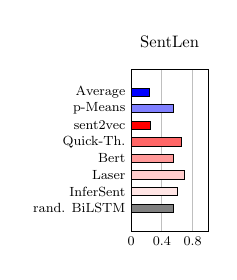
\begin{tikzpicture}[scale=0.75,every node/.style={scale=0.8}]

  	\begin{axis}[
		title=SentLen\strut,
 	   	xbar stacked,
		bar width=4pt,
		enlarge y limits=0.2,
    		symbolic y coords={rand. BiLSTM,InferSent,Laser,Bert,Quick-Th.,sent2vec,p-Means,Average},
		xmin=0,xmax=1,
  		xmajorgrids,
		tickwidth=0pt,
		xtick distance=0.40,
  		ytick=data,
		scale only axis=true,
  		width=1.3cm,height=2.75cm,
		tick label style={font=\footnotesize}
  	]

		% Average
  		\addplot[blue,fill,draw=black] coordinates
  			{(0.240,Average) (0.00,p-Means) (0.00,sent2vec) (0.00,Quick-Th.) (0.00,Bert) (0.00,Laser) (0.00,InferSent) (0.00,rand. BiLSTM)};
		% p-Means
		\addplot[blue!50,fill,draw=black] coordinates
			{(0.00,Average) (0.553,p-Means) (0.00,sent2vec) (0.00,Quick-Th.) (0.00,Bert) (0.00,Laser) (0.00,InferSent) (0.00,rand. BiLSTM)};

		% sent2vec
		\addplot[red,fill,draw=black] coordinates 
			{(0.00,Average) (0.00,p-Means) (0.254,sent2vec) (0.00,Quick-Th.) (0.00,Bert) (0.00,Laser) (0.00,InferSent) (0.00,rand. BiLSTM)};
		% Quick-Th.
		\addplot[red!60,fill,draw=black] coordinates
			{(0.00,Average) (0.00,p-Means) (0.00,sent2vec) (0.649,Quick-Th.) (0.00,Bert) (0.00,Laser) (0.00,InferSent) (0.00,rand. BiLSTM)};
		% Bert
		\addplot[red!40,fill,draw=black] coordinates
			{(0.00,Average) (0.00,p-Means) (0.00,sent2vec) (0.00,Quick-Th.) (0.551,Bert) (0.00,Laser) (0.00,InferSent) (0.00,rand. BiLSTM)};
		% Laser
		\addplot[red!20,fill,draw=black] coordinates
			{(0.00,Average) (0.00,p-Means) (0.00,sent2vec) (0.00,Quick-Th.) (0.00,Bert) (0.697,Laser) (0.00,InferSent) (0.00,rand. BiLSTM)};
		% InferSentent
		\addplot[red!10,fill,draw=black] coordinates
			{(0.00,Average) (0.00,p-Means) (0.00,sent2vec) (0.00,Quick-Th.) (0.00,Bert) (0.00,Laser) (0.600,InferSent) (0.00,rand. BiLSTM)};

		% rand lstm
		\addplot[gray,fill,draw=black] coordinates 
			{(0.00,Average) (0.00,p-Means) (0.00,sent2vec) (0.00,Quick-Th.) (0.00,Bert) (0.00,Laser) (0.00,InferSent) (0.549,rand. BiLSTM)};

  	\end{axis}

\end{tikzpicture}
\end{minipage}
\hspace*{17mm}
\begin{minipage}{0.09\textwidth}
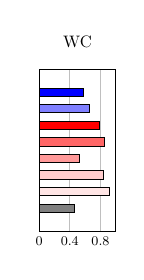
\begin{tikzpicture}[scale=0.75,every node/.style={scale=0.8}]

  	\begin{axis}[
		title=WC\strut,
   	 	xbar stacked,
		bar width=4pt,
		enlarge y limits=0.2,
	    	symbolic y coords={rand. BiLSTM,InferSent,Laser,Bert,Quick-Th.,sent2vec,p-Means,Average},
		xmin=0,xmax=1,
  		xmajorgrids,
		tickwidth=0pt,
		xtick distance=0.40,
  		ytick=data,
		yticklabels={,,},
		scale only axis=true,
  		width=1.3cm,height=2.75cm,
		tick label style={font=\footnotesize}
  	]

		% Average
  		\addplot[blue,fill,draw=black] coordinates
  			{(0.581,Average) (0.00,p-Means) (0.00,sent2vec) (0.00,Quick-Th.) (0.00,Bert) (0.00,Laser) (0.00,InferSent) (0.00,rand. BiLSTM)};
		% p-Means
		\addplot[blue!50,fill,draw=black] coordinates
			{(0.00,Average) (0.657,p-Means) (0.00,sent2vec) (0.00,Quick-Th.) (0.00,Bert) (0.00,Laser) (0.00,InferSent) (0.00,rand. BiLSTM)};

		% sent2vec
		\addplot[red,fill,draw=black] coordinates 
			{(0.00,Average) (0.00,p-Means) (0.786,sent2vec) (0.00,Quick-Th.) (0.00,Bert) (0.00,Laser) (0.00,InferSent) (0.00,rand. BiLSTM)};
		% Quick-Th.
		\addplot[red!60,fill,draw=black] coordinates
			{(0.00,Average) (0.00,p-Means) (0.00,sent2vec) (0.848,Quick-Th.) (0.00,Bert) (0.00,Laser) (0.00,InferSent) (0.00,rand. BiLSTM)};
		% Bert
		\addplot[red!40,fill,draw=black] coordinates
			{(0.00,Average) (0.00,p-Means) (0.00,sent2vec) (0.00,Quick-Th.) (0.531,Bert) (0.00,Laser) (0.00,InferSent) (0.00,rand. BiLSTM)};
		% Laser
		\addplot[red!20,fill,draw=black] coordinates
			{(0.00,Average) (0.00,p-Means) (0.00,sent2vec) (0.00,Quick-Th.) (0.00,Bert) (0.832,Laser) (0.00,InferSent) (0.00,rand. BiLSTM)};
		% InferSentent
		\addplot[red!10,fill,draw=black] coordinates
			{(0.00,Average) (0.00,p-Means) (0.00,sent2vec) (0.00,Quick-Th.) (0.00,Bert) (0.00,Laser) (0.919,InferSent) (0.00,rand. BiLSTM)};

		% rand lstm
		\addplot[gray,fill,draw=black] coordinates 
			{(0.00,Average) (0.00,p-Means) (0.00,sent2vec) (0.00,Quick-Th.) (0.00,Bert) (0.00,Laser) (0.00,InferSent) (0.462,rand. BiLSTM)};

  	\end{axis}

\end{tikzpicture}
\end{minipage}
\hspace*{10mm}
\begin{minipage}{0.09\textwidth}
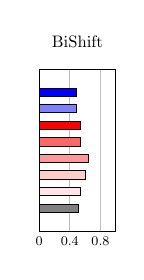
\begin{tikzpicture}[scale=0.75,every node/.style={scale=0.8}]

  	\begin{axis}[
		title=BiShift\strut,
 	   	xbar stacked,
		bar width=4pt,
		enlarge y limits=0.2,
    		symbolic y coords={rand. BiLSTM,InferSent,Laser,Bert,Quick-Th.,sent2vec,p-Means,Average},
		xmin=0,xmax=1,
  		xmajorgrids,
		tickwidth=0pt,
		xtick distance=0.40,
  		ytick=data,
		yticklabels={,,},
		scale only axis=true,
  		width=1.3cm,height=2.75cm,
		tick label style={font=\footnotesize}
  	]

		% Average
  		\addplot[blue,fill,draw=black] coordinates
  			{(0.485,Average) (0.00,p-Means) (0.00,sent2vec) (0.00,Quick-Th.) (0.00,Bert) (0.00,Laser) (0.00,InferSent) (0.00,rand. BiLSTM)};
		% p-Means
		\addplot[blue!50,fill,draw=black] coordinates
			{(0.00,Average) (0.491,p-Means) (0.00,sent2vec) (0.00,Quick-Th.) (0.00,Bert) (0.00,Laser) (0.00,InferSent) (0.00,rand. BiLSTM)};

		% sent2vec
		\addplot[red,fill,draw=black] coordinates 
			{(0.00,Average) (0.00,p-Means) (0.534,sent2vec) (0.00,Quick-Th.) (0.00,Bert) (0.00,Laser) (0.00,InferSent) (0.00,rand. BiLSTM)};
		% Quick-Th.
		\addplot[red!60,fill,draw=black] coordinates
			{(0.00,Average) (0.00,p-Means) (0.00,sent2vec) (0.544,Quick-Th.) (0.00,Bert) (0.00,Laser) (0.00,InferSent) (0.00,rand. BiLSTM)};
		% Bert
		\addplot[red!40,fill,draw=black] coordinates
			{(0.00,Average) (0.00,p-Means) (0.00,sent2vec) (0.00,Quick-Th.) (0.641,Bert) (0.00,Laser) (0.00,InferSent) (0.00,rand. BiLSTM)};
		% Laser
		\addplot[red!20,fill,draw=black] coordinates
			{(0.00,Average) (0.00,p-Means) (0.00,sent2vec) (0.00,Quick-Th.) (0.00,Bert) (0.600,Laser) (0.00,InferSent) (0.00,rand. BiLSTM)};
		% InferSentent
		\addplot[red!10,fill,draw=black] coordinates
			{(0.00,Average) (0.00,p-Means) (0.00,sent2vec) (0.00,Quick-Th.) (0.00,Bert) (0.00,Laser) (0.536,InferSent) (0.00,rand. BiLSTM)};

		% rand lstm
		\addplot[gray,fill,draw=black] coordinates 
			{(0.00,Average) (0.00,p-Means) (0.00,sent2vec) (0.00,Quick-Th.) (0.00,Bert) (0.00,Laser) (0.00,InferSent) (0.510,rand. BiLSTM)};

  	\end{axis}

\end{tikzpicture}
\end{minipage}
\hspace*{10mm}
\begin{minipage}{0.09\textwidth}
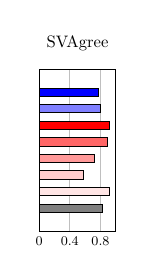
\begin{tikzpicture}[scale=0.75,every node/.style={scale=0.8}]

  	\begin{axis}[
		title=SVAgree\strut,
 	   	xbar stacked,
		bar width=4pt,
		enlarge y limits=0.2,
    		symbolic y coords={rand. BiLSTM,InferSent,Laser,Bert,Quick-Th.,sent2vec,p-Means,Average},
		xmin=0,xmax=1,
  		xmajorgrids,
		tickwidth=0pt,
		xtick distance=0.40,
  		ytick=data,
		yticklabels={,,},
		scale only axis=true,
  		width=1.3cm,height=2.75cm,
		tick label style={font=\footnotesize}
  	]

		% Average
  		\addplot[blue,fill,draw=black] coordinates
  			{(0.775,Average) (0.00,p-Means) (0.00,sent2vec) (0.00,Quick-Th.) (0.00,Bert) (0.00,Laser) (0.00,InferSent) (0.00,rand. BiLSTM)};
		% p-Means
		\addplot[blue!50,fill,draw=black] coordinates
			{(0.00,Average) (0.804,p-Means) (0.00,sent2vec) (0.00,Quick-Th.) (0.00,Bert) (0.00,Laser) (0.00,InferSent) (0.00,rand. BiLSTM)};

		% sent2vec
		\addplot[red,fill,draw=black] coordinates 
			{(0.00,Average) (0.00,p-Means) (0.910,sent2vec) (0.00,Quick-Th.) (0.00,Bert) (0.00,Laser) (0.00,InferSent) (0.00,rand. BiLSTM)};
		% Quick-Th.
		\addplot[red!60,fill,draw=black] coordinates
			{(0.00,Average) (0.00,p-Means) (0.00,sent2vec) (0.887,Quick-Th.) (0.00,Bert) (0.00,Laser) (0.00,InferSent) (0.00,rand. BiLSTM)};
		% Bert
		\addplot[red!40,fill,draw=black] coordinates
			{(0.00,Average) (0.00,p-Means) (0.00,sent2vec) (0.00,Quick-Th.) (0.718,Bert) (0.00,Laser) (0.00,InferSent) (0.00,rand. BiLSTM)};
		% Laser
		\addplot[red!20,fill,draw=black] coordinates
			{(0.00,Average) (0.00,p-Means) (0.00,sent2vec) (0.00,Quick-Th.) (0.00,Bert) (0.572,Laser) (0.00,InferSent) (0.00,rand. BiLSTM)};
		% InferSentent
		\addplot[red!10,fill,draw=black] coordinates
			{(0.00,Average) (0.00,p-Means) (0.00,sent2vec) (0.00,Quick-Th.) (0.00,Bert) (0.00,Laser) (0.912,InferSent) (0.00,rand. BiLSTM)};

		% rand lstm
		\addplot[gray,fill,draw=black] coordinates 
			{(0.00,Average) (0.00,p-Means) (0.00,sent2vec) (0.00,Quick-Th.) (0.00,Bert) (0.00,Laser) (0.00,InferSent) (0.819,rand. BiLSTM)};

  	\end{axis}

\end{tikzpicture}
\end{minipage}

\vspace*{3mm}
\begin{minipage}{0.09\textwidth}
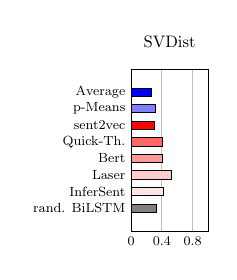
\begin{tikzpicture}[scale=0.75,every node/.style={scale=0.8}]

  	\begin{axis}[
		title=SVDist\strut,
 	   	xbar stacked,
		bar width=4pt,
		enlarge y limits=0.2,
    		symbolic y coords={rand. BiLSTM,InferSent,Laser,Bert,Quick-Th.,sent2vec,p-Means,Average},
		xmin=0,xmax=1,
  		xmajorgrids,
		tickwidth=0pt,
		xtick distance=0.40,
  		ytick=data,
		scale only axis=true,
  		width=1.3cm,height=2.75cm,
		tick label style={font=\footnotesize}
  	]

		% Average
  		\addplot[blue,fill,draw=black] coordinates
  			{(0.265,Average) (0.00,p-Means) (0.00,sent2vec) (0.00,Quick-Th.) (0.00,Bert) (0.00,Laser) (0.00,InferSent) (0.00,rand. BiLSTM)};
		% p-Means
		\addplot[blue!50,fill,draw=black] coordinates
			{(0.00,Average) (0.309,p-Means) (0.00,sent2vec) (0.00,Quick-Th.) (0.00,Bert) (0.00,Laser) (0.00,InferSent) (0.00,rand. BiLSTM)};

		% sent2vec
		\addplot[red,fill,draw=black] coordinates 
			{(0.00,Average) (0.00,p-Means) (0.301,sent2vec) (0.00,Quick-Th.) (0.00,Bert) (0.00,Laser) (0.00,InferSent) (0.00,rand. BiLSTM)};
		% Quick-Th.
		\addplot[red!60,fill,draw=black] coordinates
			{(0.00,Average) (0.00,p-Means) (0.00,sent2vec) (0.410,Quick-Th.) (0.00,Bert) (0.00,Laser) (0.00,InferSent) (0.00,rand. BiLSTM)};
		% Bert
		\addplot[red!40,fill,draw=black] coordinates
			{(0.00,Average) (0.00,p-Means) (0.00,sent2vec) (0.00,Quick-Th.) (0.406,Bert) (0.00,Laser) (0.00,InferSent) (0.00,rand. BiLSTM)};
		% Laser
		\addplot[red!20,fill,draw=black] coordinates
			{(0.00,Average) (0.00,p-Means) (0.00,sent2vec) (0.00,Quick-Th.) (0.00,Bert) (0.521,Laser) (0.00,InferSent) (0.00,rand. BiLSTM)};
		% InferSentent
		\addplot[red!10,fill,draw=black] coordinates
			{(0.00,Average) (0.00,p-Means) (0.00,sent2vec) (0.00,Quick-Th.) (0.00,Bert) (0.00,Laser) (0.414,InferSent) (0.00,rand. BiLSTM)};

		% rand lstm
		\addplot[gray,fill,draw=black] coordinates 
			{(0.00,Average) (0.00,p-Means) (0.00,sent2vec) (0.00,Quick-Th.) (0.00,Bert) (0.00,Laser) (0.00,InferSent) (0.323,rand. BiLSTM)};

  	\end{axis}

\end{tikzpicture}
\end{minipage}
\hspace*{19.75mm}
\begin{minipage}{0.09\textwidth}
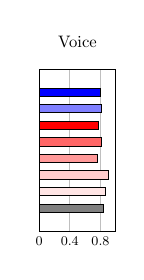
\begin{tikzpicture}[scale=0.75,every node/.style={scale=0.8}]

  	\begin{axis}[
		title=Voice\strut,
    		xbar stacked,
		bar width=4pt,
		enlarge y limits=0.2,
    		symbolic y coords={rand. BiLSTM,InferSent,Laser,Bert,Quick-Th.,sent2vec,p-Means,Average},
		xmin=0,xmax=1,
  		xmajorgrids,
		tickwidth=0pt,
		xtick distance=0.40,
  		ytick=data,
		yticklabels={,,},
		scale only axis=true,
  		width=1.3cm,height=2.75cm,
		tick label style={font=\footnotesize}
  	]

		% Average
  		\addplot[blue,fill,draw=black] coordinates
  			{(0.798,Average) (0.00,p-Means) (0.00,sent2vec) (0.00,Quick-Th.) (0.00,Bert) (0.00,Laser) (0.00,InferSent) (0.00,rand. BiLSTM)};
		% p-Means
		\addplot[blue!50,fill,draw=black] coordinates
			{(0.00,Average) (0.807,p-Means) (0.00,sent2vec) (0.00,Quick-Th.) (0.00,Bert) (0.00,Laser) (0.00,InferSent) (0.00,rand. BiLSTM)};

		% sent2vec
		\addplot[red,fill,draw=black] coordinates 
			{(0.00,Average) (0.00,p-Means) (0.779,sent2vec) (0.00,Quick-Th.) (0.00,Bert) (0.00,Laser) (0.00,InferSent) (0.00,rand. BiLSTM)};
		% Quick-Th.
		\addplot[red!60,fill,draw=black] coordinates
			{(0.00,Average) (0.00,p-Means) (0.00,sent2vec) (0.811,Quick-Th.) (0.00,Bert) (0.00,Laser) (0.00,InferSent) (0.00,rand. BiLSTM)};
		% Bert
		\addplot[red!40,fill,draw=black] coordinates
			{(0.00,Average) (0.00,p-Means) (0.00,sent2vec) (0.00,Quick-Th.) (0.760,Bert) (0.00,Laser) (0.00,InferSent) (0.00,rand. BiLSTM)};
		% Laser
		\addplot[red!20,fill,draw=black] coordinates
			{(0.00,Average) (0.00,p-Means) (0.00,sent2vec) (0.00,Quick-Th.) (0.00,Bert) (0.904,Laser) (0.00,InferSent) (0.00,rand. BiLSTM)};
		% InferSentent
		\addplot[red!10,fill,draw=black] coordinates
			{(0.00,Average) (0.00,p-Means) (0.00,sent2vec) (0.00,Quick-Th.) (0.00,Bert) (0.00,Laser) (0.868,InferSent) (0.00,rand. BiLSTM)};

		% rand lstm
		\addplot[gray,fill,draw=black] coordinates 
			{(0.00,Average) (0.00,p-Means) (0.00,sent2vec) (0.00,Quick-Th.) (0.00,Bert) (0.00,Laser) (0.00,InferSent) (0.833,rand. BiLSTM)};

  	\end{axis}

\end{tikzpicture}
\end{minipage}
\hspace*{10mm}
\begin{minipage}{0.09\textwidth}
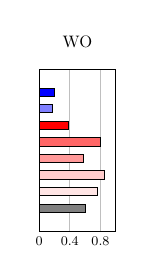
\begin{tikzpicture}[scale=0.75,every node/.style={scale=0.8}]

  	\begin{axis}[
		title=WO\strut,
   	 	xbar stacked,
		bar width=4pt,
		enlarge y limits=0.2,
    		symbolic y coords={rand. BiLSTM,InferSent,Laser,Bert,Quick-Th.,sent2vec,p-Means,Average},
		xmin=0,xmax=1,
  		xmajorgrids,
		tickwidth=0pt,
		xtick distance=0.40,
  		ytick=data,
		yticklabels={,,},
		scale only axis=true,
  		width=1.3cm,height=2.75cm,
		tick label style={font=\footnotesize}
  	]

		% Average
  		\addplot[blue,fill,draw=black] coordinates
  			{(0.201,Average) (0.00,p-Means) (0.00,sent2vec) (0.00,Quick-Th.) (0.00,Bert) (0.00,Laser) (0.00,InferSent) (0.00,rand. BiLSTM)};
		% p-Means
		\addplot[blue!50,fill,draw=black] coordinates
			{(0.00,Average) (0.173,p-Means) (0.00,sent2vec) (0.00,Quick-Th.) (0.00,Bert) (0.00,Laser) (0.00,InferSent) (0.00,rand. BiLSTM)};

		% sent2vec
		\addplot[red,fill,draw=black] coordinates 
			{(0.00,Average) (0.00,p-Means) (0.381,sent2vec) (0.00,Quick-Th.) (0.00,Bert) (0.00,Laser) (0.00,InferSent) (0.00,rand. BiLSTM)};
		% Quick-Th.
		\addplot[red!60,fill,draw=black] coordinates
			{(0.00,Average) (0.00,p-Means) (0.00,sent2vec) (0.802,Quick-Th.) (0.00,Bert) (0.00,Laser) (0.00,InferSent) (0.00,rand. BiLSTM)};
		% Bert
		\addplot[red!40,fill,draw=black] coordinates
			{(0.00,Average) (0.00,p-Means) (0.00,sent2vec) (0.00,Quick-Th.) (0.573,Bert) (0.00,Laser) (0.00,InferSent) (0.00,rand. BiLSTM)};
		% Laser
		\addplot[red!20,fill,draw=black] coordinates
			{(0.00,Average) (0.00,p-Means) (0.00,sent2vec) (0.00,Quick-Th.) (0.00,Bert) (0.846,Laser) (0.00,InferSent) (0.00,rand. BiLSTM)};
		% InferSentent
		\addplot[red!10,fill,draw=black] coordinates
			{(0.00,Average) (0.00,p-Means) (0.00,sent2vec) (0.00,Quick-Th.) (0.00,Bert) (0.00,Laser) (0.760,InferSent) (0.00,rand. BiLSTM)};

		% rand lstm
		\addplot[gray,fill,draw=black] coordinates 
			{(0.00,Average) (0.00,p-Means) (0.00,sent2vec) (0.00,Quick-Th.) (0.00,Bert) (0.00,Laser) (0.00,InferSent) (0.598,rand. BiLSTM)};

  	\end{axis}

\end{tikzpicture}
\end{minipage}
\hspace*{10mm}
\begin{minipage}{0.09\textwidth}
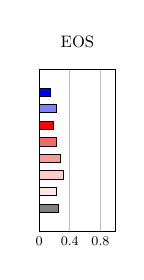
\begin{tikzpicture}[scale=0.75,every node/.style={scale=0.8}]

  	\begin{axis}[
		title=EOS\strut,
  	  	xbar stacked,
		bar width=4pt,
		enlarge y limits=0.2,
    		symbolic y coords={rand. BiLSTM,InferSent,Laser,Bert,Quick-Th.,sent2vec,p-Means,Average},
		xmin=0,xmax=1,
  		xmajorgrids,
		tickwidth=0pt,
		xtick distance=0.40,
  		ytick=data,
		yticklabels={,,},
		scale only axis=true,
  		width=1.3cm,height=2.75cm,
		tick label style={font=\footnotesize}
  	]

		% Average
  		\addplot[blue,fill,draw=black] coordinates
  			{(0.150,Average) (0.00,p-Means) (0.00,sent2vec) (0.00,Quick-Th.) (0.00,Bert) (0.00,Laser) (0.00,InferSent) (0.00,rand. BiLSTM)};
		% p-Means
		\addplot[blue!50,fill,draw=black] coordinates
			{(0.00,Average) (0.231,p-Means) (0.00,sent2vec) (0.00,Quick-Th.) (0.00,Bert) (0.00,Laser) (0.00,InferSent) (0.00,rand. BiLSTM)};

		% sent2vec
		\addplot[red,fill,draw=black] coordinates 
			{(0.00,Average) (0.00,p-Means) (0.191,sent2vec) (0.00,Quick-Th.) (0.00,Bert) (0.00,Laser) (0.00,InferSent) (0.00,rand. BiLSTM)};
		% Quick-Th.
		\addplot[red!60,fill,draw=black] coordinates
			{(0.00,Average) (0.00,p-Means) (0.00,sent2vec) (0.221,Quick-Th.) (0.00,Bert) (0.00,Laser) (0.00,InferSent) (0.00,rand. BiLSTM)};
		% Bert
		\addplot[red!40,fill,draw=black] coordinates
			{(0.00,Average) (0.00,p-Means) (0.00,sent2vec) (0.00,Quick-Th.) (0.282,Bert) (0.00,Laser) (0.00,InferSent) (0.00,rand. BiLSTM)};
		% Laser
		\addplot[red!20,fill,draw=black] coordinates
			{(0.00,Average) (0.00,p-Means) (0.00,sent2vec) (0.00,Quick-Th.) (0.00,Bert) (0.319,Laser) (0.00,InferSent) (0.00,rand. BiLSTM)};
		% InferSentent
		\addplot[red!10,fill,draw=black] coordinates
			{(0.00,Average) (0.00,p-Means) (0.00,sent2vec) (0.00,Quick-Th.) (0.00,Bert) (0.00,Laser) (0.230,InferSent) (0.00,rand. BiLSTM)};

		% rand lstm
		\addplot[gray,fill,draw=black] coordinates 
			{(0.00,Average) (0.00,p-Means) (0.00,sent2vec) (0.00,Quick-Th.) (0.00,Bert) (0.00,Laser) (0.00,InferSent) (0.246,rand. BiLSTM)};

  	\end{axis}

\end{tikzpicture}
\end{minipage}
\hspace*{10mm}
\begin{minipage}{0.09\textwidth}
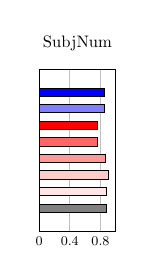
\begin{tikzpicture}[scale=0.75,every node/.style={scale=0.8}]

  	\begin{axis}[
		title=SubjNum\strut,
    		xbar stacked,
		bar width=4pt,
		enlarge y limits=0.2,
    		symbolic y coords={rand. BiLSTM,InferSent,Laser,Bert,Quick-Th.,sent2vec,p-Means,Average},
		xmin=0,xmax=1,
  		xmajorgrids,
		tickwidth=0pt,
		xtick distance=0.40,
  		ytick=data,
		yticklabels={,,},
		scale only axis=true,
  		width=1.3cm,height=2.75cm,
		tick label style={font=\footnotesize}
  	]

		% Average
  		\addplot[blue,fill,draw=black] coordinates
  			{(0.855,Average) (0.00,p-Means) (0.00,sent2vec) (0.00,Quick-Th.) (0.00,Bert) (0.00,Laser) (0.00,InferSent) (0.00,rand. BiLSTM)};
		% p-Means
		\addplot[blue!50,fill,draw=black] coordinates
			{(0.00,Average) (0.850,p-Means) (0.00,sent2vec) (0.00,Quick-Th.) (0.00,Bert) (0.00,Laser) (0.00,InferSent) (0.00,rand. BiLSTM)};

		% sent2vec
		\addplot[red,fill,draw=black] coordinates 
			{(0.00,Average) (0.00,p-Means) (0.759,sent2vec) (0.00,Quick-Th.) (0.00,Bert) (0.00,Laser) (0.00,InferSent) (0.00,rand. BiLSTM)};
		% Quick-Th.
		\addplot[red!60,fill,draw=black] coordinates
			{(0.00,Average) (0.00,p-Means) (0.00,sent2vec) (0.758,Quick-Th.) (0.00,Bert) (0.00,Laser) (0.00,InferSent) (0.00,rand. BiLSTM)};
		% Bert
		\addplot[red!40,fill,draw=black] coordinates
			{(0.00,Average) (0.00,p-Means) (0.00,sent2vec) (0.00,Quick-Th.) (0.858,Bert) (0.00,Laser) (0.00,InferSent) (0.00,rand. BiLSTM)};
		% Laser
		\addplot[red!20,fill,draw=black] coordinates
			{(0.00,Average) (0.00,p-Means) (0.00,sent2vec) (0.00,Quick-Th.) (0.00,Bert) (0.899,Laser) (0.00,InferSent) (0.00,rand. BiLSTM)};
		% InferSentent
		\addplot[red!10,fill,draw=black] coordinates
			{(0.00,Average) (0.00,p-Means) (0.00,sent2vec) (0.00,Quick-Th.) (0.00,Bert) (0.00,Laser) (0.879,InferSent) (0.00,rand. BiLSTM)};

		% rand lstm
		\addplot[gray,fill,draw=black] coordinates 
			{(0.00,Average) (0.00,p-Means) (0.00,sent2vec) (0.00,Quick-Th.) (0.00,Bert) (0.00,Laser) (0.00,InferSent) (0.879,rand. BiLSTM)};

  	\end{axis}

\end{tikzpicture}
\end{minipage}